%!TEX root = main.tex

%=================TD functions==================
\def\boldcommandlist{\@elt OP,\@elt OPs,}
\def\@elt#1,{%
 \expandafter\def\csname#1\endcsname{\textbf{#1}\xspace}
}
\boldcommandlist

\def\topColorList{\@elt TOP,\@elt TOPs,}
\def\@elt#1,{%
 \expandafter\def\csname#1\endcsname{\textcolor{TOP}{\textbf{#1}}\xspace}
}
\topColorList

\def\chopColorList{\@elt CHOP,\@elt CHOPs,}
\def\@elt#1,{%
 \expandafter\def\csname#1\endcsname{\textcolor{CHOP}{\textbf{#1}}\xspace}
}
\chopColorList

\def\sopColorList{\@elt SOP,\@elt SOPs,}
\def\@elt#1,{%
 \expandafter\def\csname#1\endcsname{\textcolor{SOP}{\textbf{#1}}\xspace}
}
\sopColorList

\def\datColorList{\@elt DAT,\@elt DATs,}
\def\@elt#1,{%
 \expandafter\def\csname#1\endcsname{\textcolor{DAT}{\textbf{#1}}\xspace}
}
\datColorList

\def\matColorList{\@elt MAT,\@elt MATs,}
\def\@elt#1,{%
 \expandafter\def\csname#1\endcsname{\textcolor{MAT}{\textbf{#1}}\xspace}
}
\matColorList


\def\compColorList{\@elt COMP,\@elt COMPs,}
\def\@elt#1,{%
 \expandafter\def\csname#1\endcsname{\textcolor{COMP}{\textbf{#1}}\xspace}
}
\compColorList

\def\redcommandlist{\@elt missingImage,}
\def\@elt#1,{%
 \expandafter\def\csname#1\endcsname{\textcolor{red}{\textbf{#1}}\xspace}
}
\redcommandlist

%===============================================

\chapter{Lecture 5}

\section*{Notes}

\section*{Contents}

\subsection*{Pitch Visualization (Bach Piece)} % (fold)
\subsection*{Communication with Max/MSP} % (fold)
\subsection*{Projection Mapping} % (fold)
\subsection*{GLSL}
\subsection*{Procedural Modeling} % (fold)
https://www.shadertoy.com/view/MdfBRX

\label{sub:procedural_modeling}

\begin{itemize}
	\item group SOP
	\item latice SOP
	\item magnet/force/metaball SOP
	\item Texture SOP
	\item Model SOP
\end{itemize}

\section{Projection Mapping}
\link{https://docs.derivative.ca/index.php?title=Projection\_mapping}{Projection Mapping}

\subsection{2D Mapping}
There are a couple of \TOPs that enable us to do simple mapping tasks:
\begin{itemize}
	\item \refTOP{Crop}
	\item \refTOP{Corner\_Pin}
	\item \refTOP{Transform}
	\item \refTOP{Displace}
\end{itemize}
So if we jsut need some slight adjustment of our output we can come up with our own mapping tool. This keeps our network simple and is a good choice if we need nothing fancy.\\
For more complex 2D mapping scenarios TouchDesiger comes with some pretty advanced tools that helps us to properly map one or multiple textures to the physical environment.

\subsubsection{Stoner}
The \link{https://docs.derivative.ca/index.php?title=Palette:Stoner}{Stoner} \COMP can be found in the Palette.

\begin{figure}[H]
	\centering
	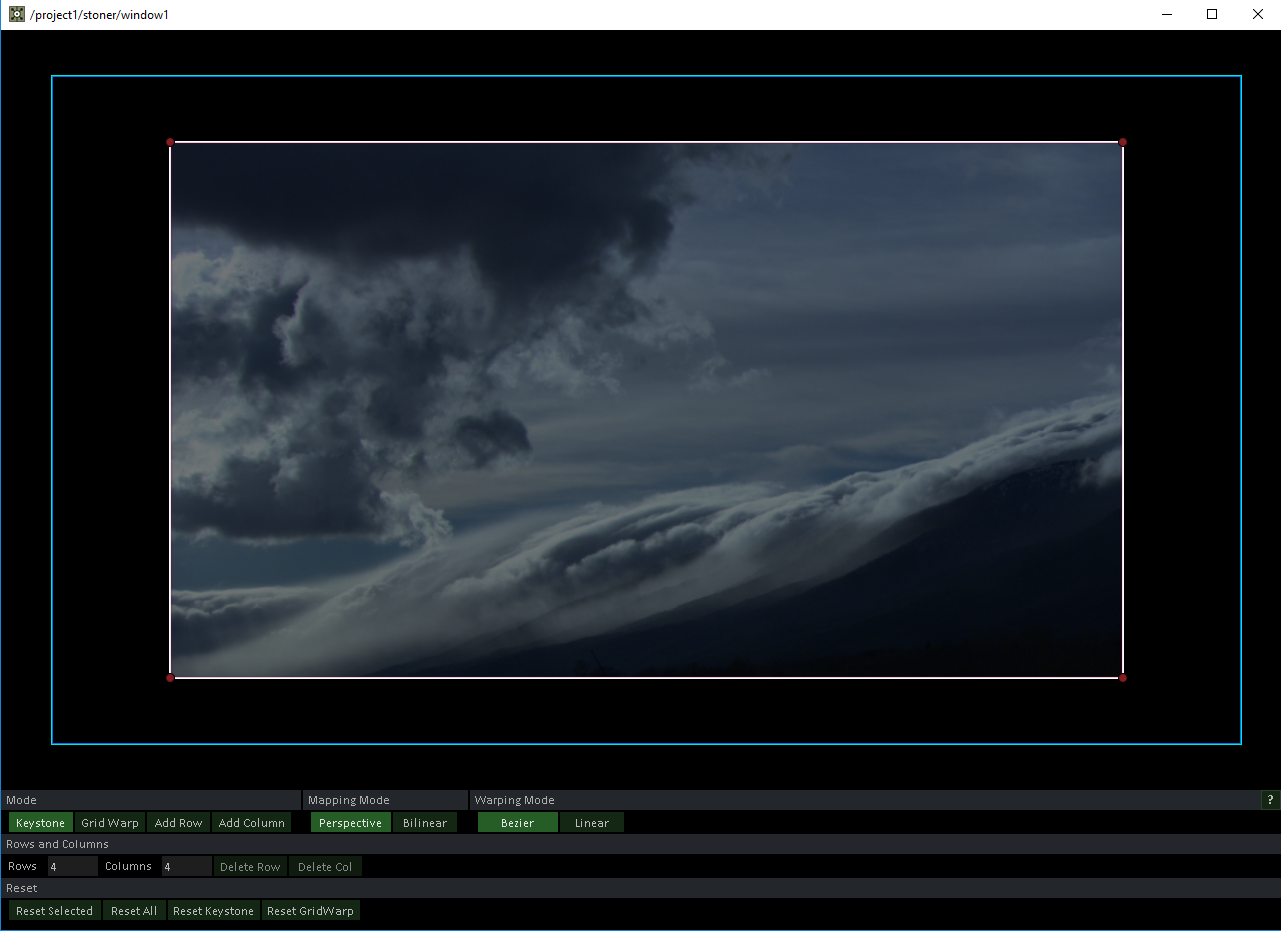
\includegraphics[width=\textwidth]{img/stoner.PNG}
	\caption[shortCaption]
	{CAPTION MISSING}
	\label{fig:label}
\end{figure}

\subsubsection{Kantan Mapper}
The \link{https://docs.derivative.ca/index.php?title=Palette:kantanMapper}{Kantan Mapper} \COMP can be found in the Palette.


\begin{figure}[H]
	\centering
	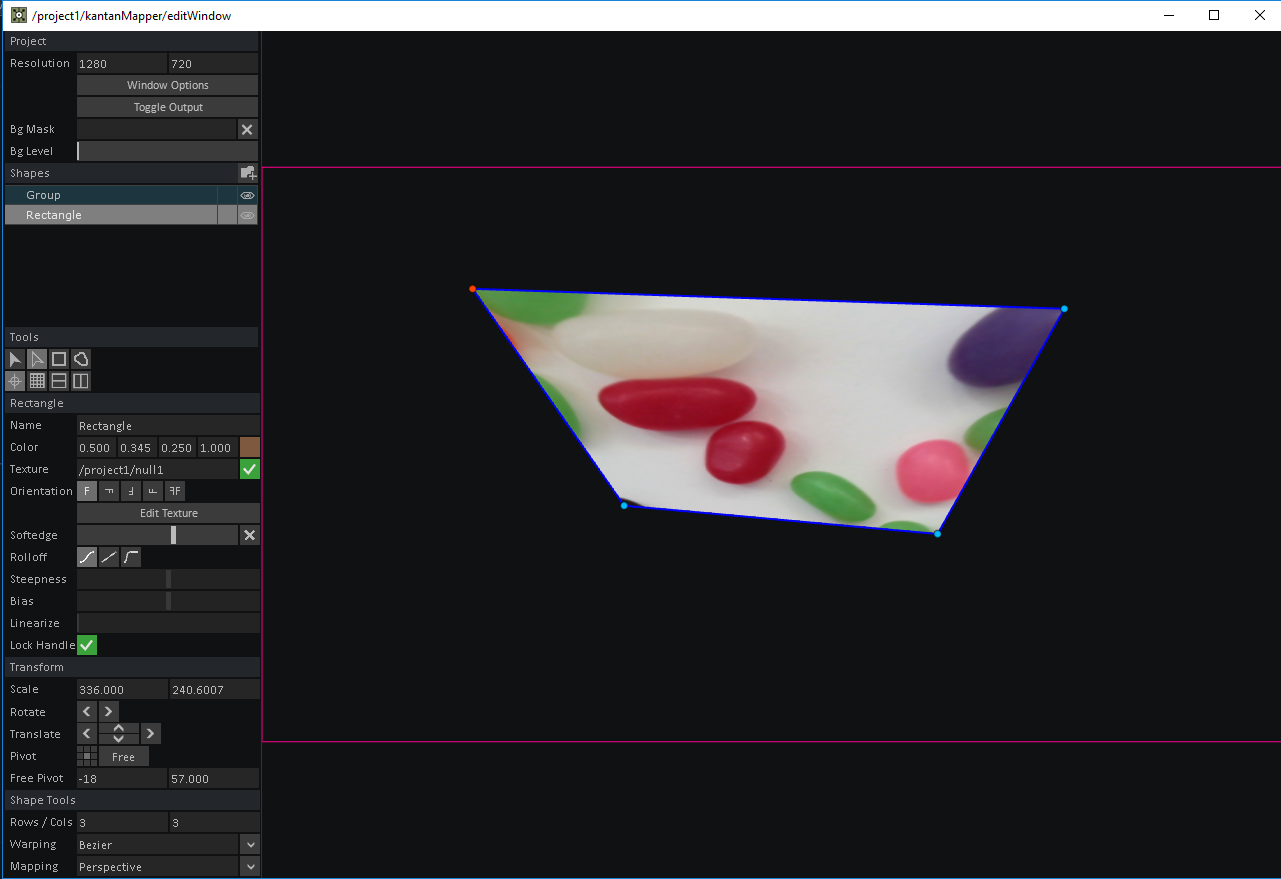
\includegraphics[width=\textwidth]{img/kantanMapper.PNG}
	\caption[shortCaption]
	{CAPTION MISSING}
	\label{fig:label}
\end{figure}

\subsubsection{External Tools}
Also we can use other tools than TouchDesigner for mapping. We can send our video material to other software packages via the \refTOP{DirectX\_Out} or the \refTOP{Syphon\_Spout\_Out}. Popular mapping tools are for example:
\begin{itemize}
	\item \link{https://madmapper.com/}{Madmapper}
	\item \link{https://visution.com/}{Visution MAPIO2}
	\item \link{https://resolume.com/software}{Resolume Arena}
	\item \link{https://troikatronix.com/}{Isadora}
\end{itemize}


\subsection{3D Mapping}
For 3D mapping, we need a 3D model of the physical structure we want to be mapped. Obviously, two scenartios could come about here:
\begin{enumerate}
	\item Either we start with a 3d Model and Build it in reality or
	\item  we start from a physical Object and create a 3D model of it.
\end{enumerate}
For scenario 1, we could start off in a CAD program like Solid Works or Auto CAD, design a structure and build it/3D-print it.
In Scenario two we are confronted with a physical object and need to get an accurate 3D model of it. Sometimes we can obtain construction plans and accurately rebuild the object this way. In other cases we need to somehow measure the object, since there are no plans. This can be done using a laser or using photogrammetry. Autodesk provides software that does this(\link{https://www.autodesk.com/products/recap/overview}{Recap}), but there are many programs that try to extract a 3D model from a series of photos or a video like \link{http://ccwu.me/vsfm/}{VisualSFM}.\\

When we have a 3D Model of the structure we want to map we can use CamSchnappr in TouchDesigner to automatically estimate the objects position, the projectors position and the lens parameters of the projector to automatically align our projection with the physical world.
The \link{https://docs.derivative.ca/index.php?title=Palette:CamSchnappr}{CamSchnappr} \COMP can be found in the Palette.


% subsection scripting (end)
% subsection procedural_modeling (end)

\section{GLSL}
GLSL is a C-style language. It enables us to write code that runs on the GPU. Since the GPU has a massively parallelized architecture, some processes can be faster to calculate on it by a huge margin.\\
In TouchDesigner we have a couple of ways to write such a program wich is typically called a \textit{Shader}\index{Shader}\footnote{If you want a more exact definition of the word shader, go \href{https://www.khronos.org/opengl/wiki/OpenGL_Shading_Language}{here}}. We shouldn't forget though, that all \TOPs \textit{are} shaders and calculated on the GPU and \MATs are as well.\\
But if we want to write GLSL code we can do so by using the following \OPs:
\begin{itemize}
	\item \refTOP{GLSL}
	\item \refTOP{GLSL\_Multi}
	\item GLSL \MAT
\end{itemize}
Also, the \link{https://docs.derivative.ca/index.php?title=GLSL}{GLSL Wiki page} is a good starting place to get oriented how to write shaders in TD.\\


Learning how to code in GLSL is out of the scope of this course. But we will go ahead and use some shader code we find online and slightly change it so it runs inside TouchDesigner. A highly recommended resource for learning how to write GLSL is \link{https://thebookofshaders.com/}{The Book of Shaders}. Another interesting resource is \link{https://www.shadertoy.com/}{Shadertoy}. Here we can find tons of shaders and look at them online. We can then just grab the code and port it to TouchDesigner, which is what we are going to do next.\\

I more or less randomly picked a shader from Shadertoy, \link{https://www.shadertoy.com/view/Ms2SD1}{this one}. Its output looks like this:

\begin{figure}[H]
	\centering
	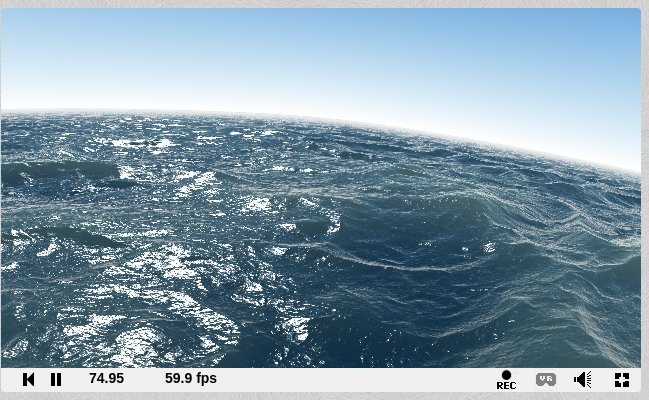
\includegraphics[width=\textwidth]{img/sea.png}
	\caption[shortCaption]
	{CAPTION MISSING}
	\label{fig:label}
\end{figure}

And its code looks like this (don't panic now):

\lstinputlisting[language=C, numbers=left,firstline=0]{code/seascape.frag}


So, we can put down a GLSL \TOP in TouchDesigner and can just copy paste the code into the Text \DAT called \texttt{glsl1\_pixel} that should be attached to the GLSL \TOP. Just copy the contents of the file above what's in there already. When we did that, we see a couple of errors.

